\documentclass[10pt,a4paper]{article}

\usepackage[margin=0.68in]{geometry}
\usepackage[T1]{fontenc}
\usepackage[utf8]{inputenc}
\usepackage{lmodern}
\usepackage{microtype}
\usepackage{booktabs}
\usepackage{tabularx}
\usepackage{array}
\usepackage{float}
\usepackage{enumitem}
\usepackage{xcolor}
\usepackage{hyperref}
\usepackage{tikz}
\usetikzlibrary{arrows.meta,positioning,shapes.geometric}

\hypersetup{
  colorlinks=true,
  linkcolor=blue!50!black,
  urlcolor=blue!50!black
}
\setlist{nosep,leftmargin=*}
\setlength{\parindent}{0pt}
\setlength{\parskip}{4pt}
\renewcommand{\arraystretch}{1.12}
\newcolumntype{L}[1]{>{\raggedright\arraybackslash}p{#1}}
\newcolumntype{Y}{>{\raggedright\arraybackslash}X}

\title{\vspace{-1.2cm}\textbf{Design Report: Urban Data Lakehouse}\\
\large ID2221 Data-Intensive Computing --- Week 1}
\author{ID2221 Project Team}
\date{September 2026}

\begin{document}
\maketitle
\vspace{-0.8cm}

\begin{abstract}
This project implements a reusable local data-engineering platform for four
heterogeneous urban datasets: NYC yellow taxi trips, taxi zones, hourly
weather, and hourly PM2.5 observations. PySpark~\cite{sparktypes} provides
distributed transformations, while Delta Lake~\cite{delta} supplies
transactional tables for the raw,
normalized, integrated, aggregate, and benchmark layers. The platform
enforces versioned source contracts, standardizes schemas and local timestamps,
quarantines invalid records, enriches each retained taxi trip with spatial and
environmental context, and produces analysis-ready Delta tables. For the
supplied Q1 2024 data, 9,551,387 cleaned trips are retained and the integration
preserves exactly the same row count.
\end{abstract}

\section{System Architecture}

The platform follows a layered lakehouse design. Source files are first copied
into immutable project storage and ingested into raw Delta tables with lineage
metadata. Dataset-specific cleaning then produces a common representation in
the normal layer. The integration layer joins taxi trips with two taxi-zone
roles and with hourly weather and air quality. Aggregate tables and alternative
physical layouts support the required analytical queries and benchmarks.

\begin{center}
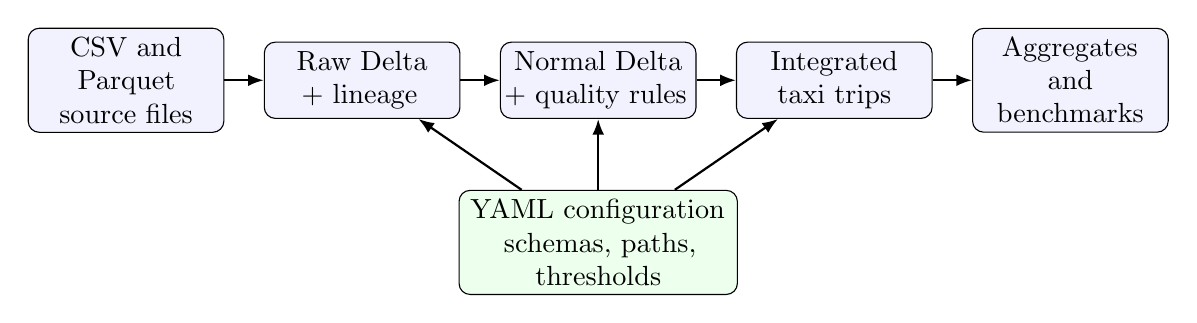
\begin{tikzpicture}[
  node distance=5mm,
  box/.style={draw, rounded corners, align=center, minimum height=9mm,
              text width=2.25cm, fill=blue!5},
  arrow/.style={-{Latex[length=2mm]}, thick}
]
  \node[box] (source) {CSV and Parquet\\source files};
  \node[box, right=of source] (raw) {Raw Delta\\+ lineage};
  \node[box, right=of raw] (normal) {Normal Delta\\+ quality rules};
  \node[box, right=of normal] (integrated) {Integrated\\taxi trips};
  \node[box, right=of integrated] (consumer) {Aggregates and\\benchmarks};
  \draw[arrow] (source) -- (raw);
  \draw[arrow] (raw) -- (normal);
  \draw[arrow] (normal) -- (integrated);
  \draw[arrow] (integrated) -- (consumer);
  \node[box, below=9mm of normal, text width=3.3cm, fill=green!7] (config)
    {YAML configuration\\schemas, paths, thresholds};
  \draw[arrow] (config) -- (raw);
  \draw[arrow] (config) -- (normal);
  \draw[arrow] (config) -- (integrated);
\end{tikzpicture}
\end{center}

The command-line entry point selects a stage, while shared helpers create the
Spark session, validate configuration, resolve schema versions and paths, and
read or write Delta tables. The scheduled \texttt{all} command always checks
sources first and rebuilds downstream layers only if at least one new valid raw
record is accepted. Benchmarking remains an explicit, independent operation.
This separation keeps orchestration thin and allows stages to be tested
independently.

\section{Data Catalog}

\begin{table}[H]
\centering
\small
\begin{tabularx}{\textwidth}{@{}L{2.5cm}L{4.0cm}Y@{}}
\toprule
\textbf{Dataset} & \textbf{Primary entity and key} & \textbf{Join and temporal attributes} \\
\midrule
Yellow taxi trips~\cite{nyctlc} & One taxi trip. The source has no stable trip identifier;
the platform uses the SHA-256 ingestion record hash as \texttt{trip\_id}. &
Joins on pickup and dropoff location IDs and on pickup hour. Pickup and dropoff
timestamps are temporal attributes. \\
Taxi zone lookup & One taxi zone, uniquely identified by
\texttt{location\_id}. & Joined twice to the taxi table through pickup and
dropoff location IDs. It has no temporal attribute. \\
Hourly weather & One weather observation per local hour, uniquely identified
by year, month, day, and hour; normalized to \texttt{event\_hour}. & Joined to
\texttt{pickup\_hour}. The source date parts and normalized timestamp are
temporal. \\
Air quality & Raw grain: one PM2.5 sensor observation. Normal grain: one NYC
hour, uniquely identified by \texttt{event\_hour}. & Raw identity includes
state, county, site, POC, parameter, and time. The hourly result joins to taxi
pickup hour. \\
\bottomrule
\end{tabularx}
\end{table}

Taxi vendor, rate code, payment type, and store-and-forward flag are
categorical. Borough, zone, and service zone are categorical lookup
attributes. Weather condition and source fields are categorical, as are air
quality geography, unit, qualifier, and measurement method. Taxi trips grow
most rapidly; weather and air quality grow hourly; the zone lookup is small and
changes infrequently. Conceptually, taxi zones, normalized hourly weather, and
normalized hourly air quality are lookup tables relative to the taxi fact
table.

\section{Storage Architecture and Naming}

All managed datasets are stored as Delta tables below
\texttt{data/lakehouse}. The raw layer preserves ingested values and lineage;
the normal layer contains typed, standardized data; the integrated layer
contains the analysis-ready wide table; and aggregate and benchmark layers
contain derived outputs. Lowercase \texttt{snake\_case} is used throughout.
Units are included in names such as \texttt{temperature\_c},
\texttt{wind\_speed\_kmh}, and \texttt{pm25\_avg\_ug\_m3}.

The large normal and integrated taxi tables are partitioned by pickup year and
month, which supports temporal pruning without creating one partition per day.
Taxi zones and weather are not partitioned because they contain only 265 and
8,784 rows respectively. The normalized air-quality table is currently
partitioned by event year and month for consistency with time-series growth,
although its present 8,784-row size means that an unpartitioned layout would
also be reasonable.

Partitioning becomes harmful when a key has high cardinality, partitions are
small, or queries do not filter on the partition column. In these cases, small
files and metadata operations can cost more than the data scan they avoid. The
benchmark therefore compares unpartitioned, borough-, month-, and date-based
layouts. Random bucket layouts with comparable target file counts help
separate the effect of semantic partitioning from the effect of file count.

\section{Reusable Ingestion Framework}

The ingestion framework discovers files from configurable paths and patterns,
loads CSV or Parquet input, verifies expected columns, converts column names to
\texttt{snake\_case}, adds lineage, and writes Delta tables. A source-file
registry records path, size, modification time, and an optional checksum so
unchanged inputs can be skipped after a successful run. Per-run metadata
records status, processed rows, rejected rows, execution time, and errors.

Generic components include file discovery, format dispatch, column-name
normalization, Delta I/O, record hashing, run tracking, schema-contract
validation, safe type conversion, and registry updates. Each dataset declares
a positive \texttt{current\_schema\_version} and retains all historical
contracts under \texttt{schema\_versions}. A contract specifies format,
expected columns, explicit column types, mappings, and read options. Parquet
physical types are checked exactly; CSV values are read without schema
inference and converted against the declared types. Missing or unexpected
columns fail the file-level contract, while row-level conversion failures are
written with their reasons to \texttt{rejected/consumption}.

Every accepted raw row, source-file registry entry, and ingestion-run record
stores the selected schema version. Changing the current-version pointer does
not silently reinterpret historical rows; a backfill is an explicit operation.
Normal tables select the latest ingestion, using schema version only as a
tie-breaker, for repeated business keys. One-record outputs preserve a scalar source
version, while multi-source or aggregated outputs preserve source-specific
versions or version sets. Adding twenty datasets would therefore primarily
require catalog entries and declarative contracts, plus small transformation
functions only where source semantics differ.

\section{Common Representation and Data Quality}

Project event timestamps are treated as New York local wall-clock values and
stored as \texttt{timestamp\_ntz}. Weather date parts are assembled directly
with \texttt{make\_timestamp\_ntz}. Air-quality timestamps combine
\texttt{date\_local} with the time component of \texttt{time\_local} and are
parsed directly with \texttt{to\_timestamp\_ntz}. Taxi pickup hours are also
constructed directly from NTZ year, month, day, and hour components. No event
time passes through Spark's zone-aware \texttt{timestamp}; consequently, the
host machine's time zone and daylight-saving transition cannot normalize a
local 02:00 value into 03:00 or merge two source hours.

Primary keys for lookup and hourly tables must exist, be non-null, and be
unique. Records that violate required-field, timestamp, project-period,
duration, measurement, or unit rules are written with reasons to
\texttt{rejected/cleaning}. Invalid optional weather measurements are instead
converted to null so the complete hourly record remains usable. Taxi pickups
are restricted to Q1 2024; trip duration must be greater than zero and at most
24 hours; and duplicate record hashes are removed. Missing, negative, or
greater than 500-mile distances become null and are flagged. Zero-distance
trips and negative financial values are retained with explicit flags because
they may represent cancellations, refunds, or adjustments rather than
ingestion errors. This preserves business events while allowing downstream
analysis to exclude them deliberately.

\section{Integration Strategy}

The taxi-zone dimension is broadcast and joined twice: once to produce pickup
zone, borough, and service zone, and once to produce the corresponding dropoff
attributes. Weather is associated by constructing the pickup's local NTZ hour
and matching it to the unique weather \texttt{event\_hour}. Direct NTZ
construction makes the join key independent of the Spark host's time zone.

The air-quality source covers the United States and contains multiple sensor
observations per hour. The transformation restricts it to available NYC
counties (Bronx, Kings, and Queens), accepts non-negative PM2.5 measurements in
a consistent unit, repairs local timestamps, and aggregates observations to a
single city-level hourly average. Minimum, maximum, observation count, and
distinct site count are retained for auditability. Hourly aggregation before
the join prevents one taxi trip from being multiplied by several sensors.

All enrichment operations are left joins: a trip remains available when
context is missing, and \texttt{weather\_available} and
\texttt{air\_quality\_available} expose coverage explicitly. Zone, weather,
and hourly air-quality tables are broadcast because they are small compared
with the taxi fact table. Validation on the supplied data produced:

\begin{center}
\begin{tabular}{@{}lr@{}}
\toprule
\textbf{Stage or check} & \textbf{Result} \\
\midrule
Raw taxi rows & 9,554,778 \\
Cleaned taxi rows & 9,551,387 \\
Integrated taxi rows & 9,551,387 \\
Pickup and dropoff zone coverage & 100\% \\
Weather and air-quality coverage & 100\% \\
\bottomrule
\end{tabular}
\end{center}

The identical clean and integrated counts demonstrate that enrichment neither
removes nor multiplies trips.

\section{Scalability, Trade-offs, and Limitations}

At twenty times the current volume, execution should move from local mode to a
multi-worker Spark deployment backed by object storage. Shuffle partitioning
should be sized to cluster capacity, incremental transformations should replace
full overwrites, and periodic compaction should control small files. Broadcast
joins should remain only while dimension tables fit safely in executor memory;
larger dimensions would use partitioned joins. Data skipping or clustering can
supplement coarse date partitioning for common filters.

The design has deliberate limitations. Hourly matching does not interpolate
conditions at the exact pickup minute. City-level PM2.5 improves temporal
coverage but hides neighborhood variation, and the provided data has no
observations for Manhattan or Staten Island. The record hash is a practical
deduplication key rather than a source-issued business identifier. Finally,
the 24-hour duration and 500-mile distance limits are configurable operational
assumptions and should be reevaluated when the domain or time range changes.
The source registry makes ingestion incremental, but accepted new input still
causes full rebuilds of normal, integrated, and aggregate tables.

\section{Conclusion}

The implementation converts heterogeneous departmental files into a
consistent, auditable Delta Lakehouse and produces an analysis-ready taxi-trip
dataset without changing its retained grain. Configuration, shared ingestion
utilities, explicit schema-version lineage, rejected-record quarantine,
time-zone-independent local timestamps, isolated transformations, and layered
storage reduce duplication and make future datasets easier to add. Remaining
production extensions include distributed object storage and compute,
incremental downstream transforms, compaction, and operational monitoring.

\begin{thebibliography}{9}
\small
\bibitem{sparktypes}
Apache Spark, \href{https://spark.apache.org/docs/latest/sql-ref-datatypes.html}
{``Data Types --- Spark SQL.''}
\bibitem{delta}
Delta Lake, \href{https://docs.delta.io/latest/index.html}
{``Delta Lake Documentation.''}
\bibitem{nyctlc}
NYC Taxi and Limousine Commission,
\href{https://www.nyc.gov/site/tlc/about/tlc-trip-record-data.page}
{``TLC Trip Record Data.''}
\end{thebibliography}

\end{document}
